\chapter{Raspberry Pi}

\section{¿Por qué Raspberry Pi?}

Los motivos por los cuales se ha utilizado una Raspberry Pi en este proyecto son claros y han sido comentados con anterioridad. Es un dispositivo portátil de un tamaño muy reducido que nos facilita mucho el poder llevarlo y poder ofrecer un servicio en cualquier lugar sin dificultades. Tiene unas prestaciones más que aceptables para un dispositivo de ese tamaño como conexiones inalámbricas de Wifi y Bluetooth integrados, cosa imprescindible para las comunicaciones con los sensores. Todo a un precio muy atractivo que lo hace asequible.  

Algunas de las especificaciones mas importantes de las Raspberry Pi 3 son las siguientes:
\begin{itemize}
\item 1.2GHz 64-bit quad-core ARMv8 CPU
\item 802.11n Wireless LAN
\item Bluetooth 4.1 y Bluetooth Low Energy (BLE)
\item 1GB RAM
\item Ethernet port
\item Micro SD card slot 
\end{itemize}

\begin{figure}[htb]
\begin{center}
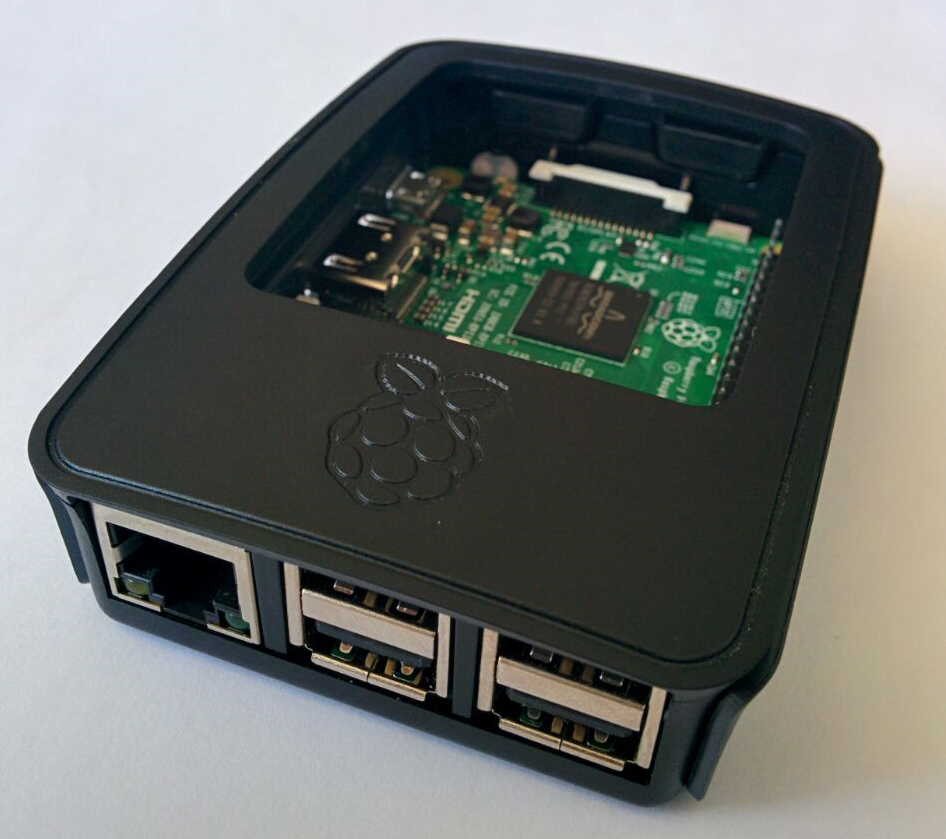
\includegraphics[width=0.65\textwidth]{./setup/raspi}
\caption{Raspberry Pi 3}
\end{center}
\end{figure}


\section{Virtualización de la Raspberry Pi}

Al inicio del proyecto no se disponía de una Raspberry Pi para poder realizar las pruebas y se decidió emularla mediante Qemu. 
Qemu es una aplicación que nos permite emular, mediante máquinas virtuales, gran parte de los sistemas operativos. 
Es realmente sencillo emular una imagen de Raspbian si no fuera por un detalle, como se comenta en el apartado 2.2: ¿Qué es Docker? Docker necesita un sistema x64 o Linux kernel 3.8+ mientras que Raspberry ejecuta un sistema ARM, lo que conlleva que Docker no sea compatible a primera instancia con la Raspberry. 
La solución para este gran problema es la utilización de Hypriot, una imagen de Raspbian modificada con Docker instalado. 
La instalación de esta imagen requiere hacer unos retoques ya que el kernel de Qemu no es del todo compatible con el de la imagen de Hypriot. Desafortunadamente, las incompatibilidades del kernel no permitían hacer un uso correcto de modo que se decidió apartar por completo la posibilidad de poder emular una Raspberry Pi con Docker instalado ya que las incompatibilidades del kernel no lo permitían.

En el apéndice se podrán ver los pasos a seguir para la instalación y emulación de la imagen. 

\section{Raspberry Pi y Docker}

Después de descartar completamente la opción de emular la imagen en Qemu se decidió probar en la Raspberry Pi de la empresa si la imagen corría correctamente. Y sí, la imagen iba perfectamente y ejecutaba Docker sin ningún problema. Contrariamente, la Raspberry Pi sí que dio problemas porque era el primer modelo, que era antiguo, y no disponía de módulos para conexiones inalámbricas integrados por lo que se decidió, aprovechando el lanzamiento de la nueva Raspberry Pi 3, comprarla ya que ésta sí dispone de de conexiones inalámbrica. 

\subsection{Instalación de la imagen en la Raspberry Pi}

Como se ha dicho, a la imagen de Raspbian no es posible instalar Docker como lo haríamos en un sistema operativo como linux. Es necesario una imagen la cual ya lo tenga instalado, como la imagen de Hypriot. La instalación se llevó a cabo de esta manera:

\begin{verbatim}
$ curl -sSL http://downloads.hypriot.com/docker-hypriot_1.8.2-1_armhf.deb 
>/tmp/docker-hypriot_1.8.2-1_armhf.deb
$ sudo dpkg -i /tmp/docker-hypriot_1.8.2-1_armhf.deb
$ rm -f /tmp/docker-hypriot_1.8.2-1_armhf.deb
$ sudo sh -c 'usermod -aG docker $SUDO_USER'
$ sudo systemctl enable docker.service
\end{verbatim}

\begin{itemize}
\item Primero descargá la imagen deseada y la montará en un directorio temporal.
\item Instalará los paquetes con el comando dpkg.
\item Borrará el archivo comprimido.
\item Ejecutará el comando donde añade el usuario a un grupo Docker. 
\item Pondrá en marcha el Daemon de Docker.  
\end{itemize}


\subsection{Creación de las imágenes de Docker}

Una vez tenemos la Raspberry lista, se pasará a la creación de las imágenes Docker para poder desplegar Aaaida.
En primer lugar se necesita un contenedor que contenga una base de datos, en este caso MongoDB. Para la creación de la imagen utilizaremos una ya creada y que esté en los repositorios de Docker Hub. Se necesita una imagen que sea compatible con ARM, cosa que no resulta sencillo ya que la gran mayoría de las imágenes no están pensadas para esta arquitectura y los pocos disponibles no estaban operativos. Otra restricción que tenemos era que debe ser una base de datos sin la necesidad de ingresar un usuario y su contraseña, cosa que no es habitual, pero que resulta una obligación en algunas imágenes.
Por lo tanto se utilizó la siguiente imagen de Docker Hub:

\begin{center}
\texttt{partlab/ubuntu-arm-mongodb}
\end{center}

La otra imagen que se utilizará será la propia de Aaaida, pero igual que, la imagen de MongoDB deberá ser compatible con una arquitectura ARM. Al ser una aplicación propia de la empresa no se encontrará en repositorios público y tendremos que crearla nosotros mediante un Dockerfile. 
En la siguiente figura se puede ver el Dockerfile que se utilizará para poder crear el contenedor con Aaaida.

\begin{verbatim}
FROM ioft/armhf-debian
RUN apt-get update; apt-get -y install curl
RUN set -ex \  
	&& for key in \    
		9554F04D7259F04124DE6B476D5A82AC7E37093B \ 
        94AE36675C464D64BAFA68DD7434390BDBE9B9C5 \
        0034A06D9D9B0064CE8ADF6BF1747F4AD2306D93 \ 
        FD3A5288F042B6850C66B31F09FE44734EB7990E \    
        71DCFD284A79C3B38668286BC97EC7A07EDE3FC1 \    
        DD8F2338BAE7501E3DD5AC78C273792F7D83545D \    
        B9AE9905FFD7803F25714661B63B535A4C206CA9 \    
        C4F0DFFF4E8C1A8236409D08E73BC641CC11F4C8 \  
	; 	do \  
		gpg --keyserver ha.pool.sks-keyservers.net --recv-keys "$key"; \  
	done

ENV NODE_VERSION 4.4.5

RUN curl -SLO 
"https://nodejs.org/dist/v$NODE_VERSION/node-v$NODE_VERSION-
linux-armv7l.tar.gz" \  
&& curl -SLO "https://nodejs.org/dist/v$NODE_VERSION/SHASUMS256.txt.asc" \  
&& gpg --batch --decrypt --output SHASUMS256.txt SHASUMS256.txt.asc \  
&& grep "node-v$NODE_VERSION-linux-armv7l.tar.gz\$" SHASUMS256.txt | 
sha256sum -c - \  
&& tar -xzf "node-v$NODE_VERSION-linux-armv7l.tar.gz" -C /usr/local 
--strip-components=1 \  
&& rm "node-v$NODE_VERSION-linux-armv7l.tar.gz" SHASUMS256.txt.asc 
SHASUMS256.txt

COPY scripts/rpi_docker/entrypoint /entrypoint
RUN mkdir /aaaida
WORKDIR /aaaida
CMD ["/entrypoint"]
EXPOSE 40000
COPY . /aaaida
\end{verbatim}

Al principio del Dockerfile se ve la acción \texttt{FROM}, encargada de cargar una imagen de una Debian para ARM. Como observación se puede detectar que la imagen del mongo es para Ubuntu ARM y la imagen base para Aaaida es una Debian ARM, distribuciones de linux diferentes en los dos contenedores. Esto demuestra que cada contenedor es un ente aislado que no tiene que depender del resto de contenedores.
 
A continuación de declarar la imagen base, vienen una serie de acciones con la instrucción \texttt{RUN}, que nos permite ejecutar cualquier comando. En el primer caso que hace un update e instala el curl.
 
Las siguientes tres instrucciones de las cuales dos de ellas son un \texttt{RUN} y la restante un \texttt{ENV}, que configura las variables de entorno, son para poder instalar el Node.js en el contenedor para poder compilar el código de Aaaida.
 
Una vez instalado se utiliza la acción \texttt{COPY}, que como su nombre indica, copiara el contenido de un directorio en un directorio del contenedor.

Si seguimos se ve que crea un directorio con el nombre de \texttt{aaaida} y hace que ese directorio sea el directorio de trabajo con la instrucción \texttt{WORKDIR}.
 
Después Ejecutará \texttt{[/entrypoint]} que al escribirlo en formato JSON la instrucción \texttt{CMD} ejecuta el contenido sin shell. El contenido de este script especifica los puertos, el host... de la aplicación. Se podrá ver su contenido en el apéndice.
 
Para terminar con las 2 últimas instrucciones, que son \texttt{EXPOSE} y \texttt{COPY}, la cual la primera indica los puertos que el contenedor tendrá activos y por los cuales escuchará. El segundo hará una copia desde el punto raíz donde se ejecutará el Dockerfile en el directorio creado anteriormente de \texttt{aaaida}.

\subsection{Despliegue de la aplicación} 

Para realizar el despliegue de Aaaida, con las dos imágenes que se han creado en el apartado anterior será suficiente. Tan solo tendremos que arrancar las imágenes para crear los contenedores. 
Primero se hará un \texttt{docker run} sobre la imagen de MongoDB y acto seguido igual con la imagen de Aaaida, pero con una pequeña diferencia: habrá que linkear el contenedor de mongo para que la aplicación pueda encontrar la base de datos necesaria para funcionar.
\pagebreak 

El comando utilizado para levantar el contenedor sería el siguiente:

\begin{center}
\begin{verbatim}
docker run --link=cc1d12ed96ee:mongo --name= aaaidaArm -e NODE_ENV=docker 
alteraid/aaaida datastore-arm
\end{verbatim}
\end{center}

En el comando se linkea el \texttt{CONTAINER ID} que sería como el número de serie del contenedor de Docker (se puede obtener usando el comando \texttt{docker ps}), también le dará un nombre al contenedor y por último el -e que permite añadir variables de entorno.
\newline 

Pero levantar los contenedores utilizando solo Docker implica estar haciendo un \texttt{run} o \texttt{start} cada vez que el servicio caiga por culpa de un apagón o fallos. Se decide instalar Docker Compose para poder orquestar las dos imágenes y añadir todas las necesidades y relaciones que necesiten. Esto permitirá tener el servicio automatizado en un fichero que tan solo habrá que arrancar una vez y en caso de fallo, el solo intentara arrancar de nuevo el servicio. El fichero utilizado se puede ver en el punto 2.5.3. Docker Compose donde también está explicado. 

Si se levanta el proceso mediante el comando \texttt{docker-compose up} se puede ver como tanto el contenedor de \texttt{aaaida} como el de \texttt{mongo} se ejecutan y tenemos la aplicación corriendo perfectamente.

\begin{figure}[htb]
\begin{center}
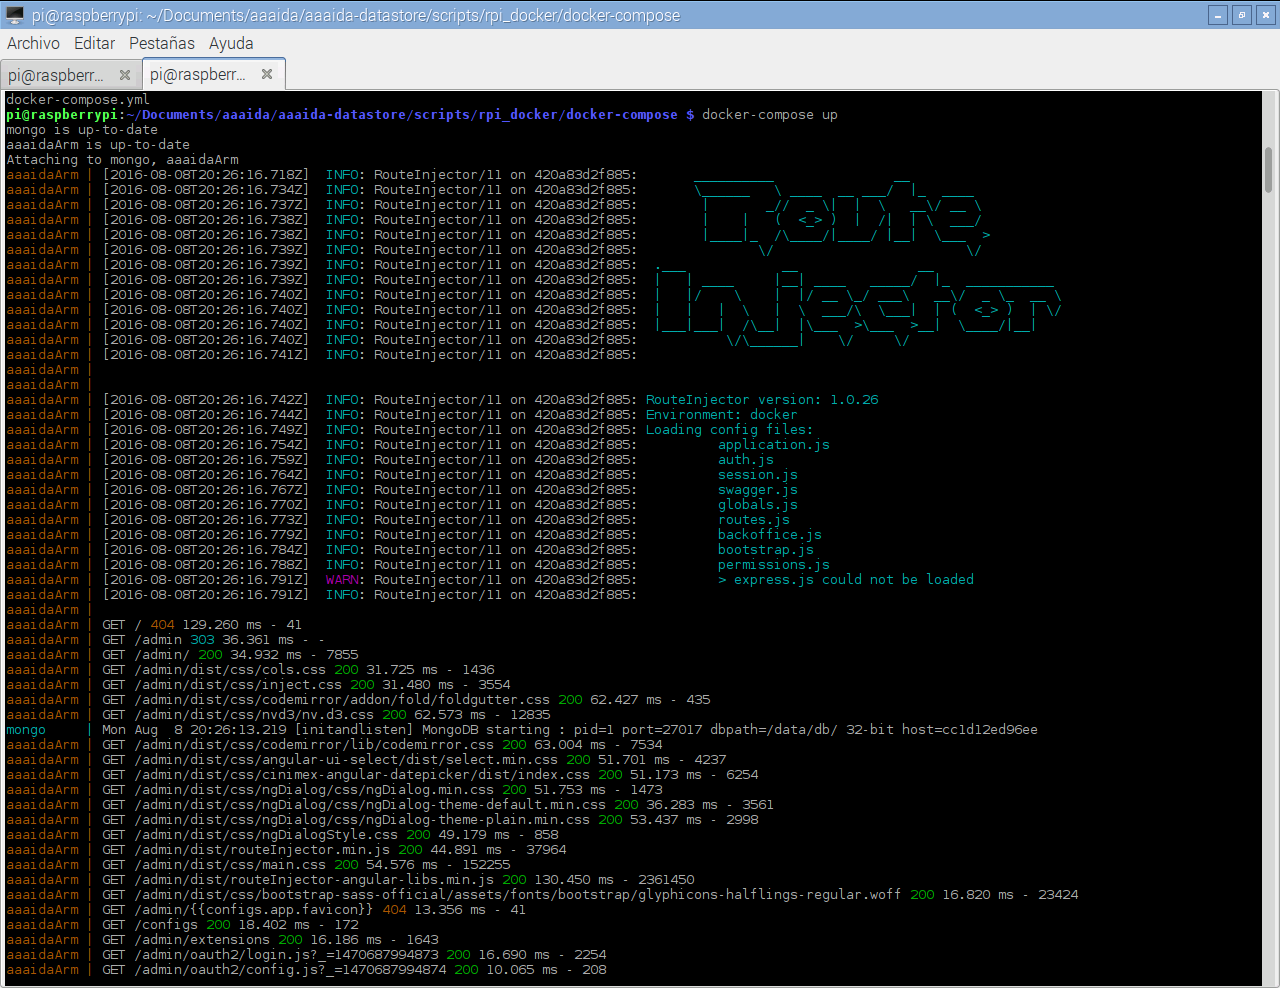
\includegraphics[width=0.95\textwidth]{./setup/dockerComposeUp}
\caption{Docker-compose up}
\label{ComUp:composeUp}
\end{center}
\end{figure} 
\pagebreak

\begin{figure}[htb]
\begin{center}
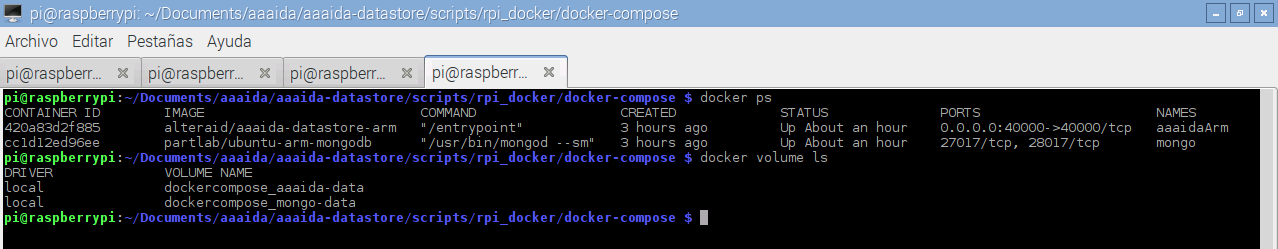
\includegraphics[width=0.95\textwidth]{./setup/dockerpsVolumen}
\caption{Listado de contenedores y volúmenes}
\label{psVl:psVolumen}
\end{center}
\end{figure} 

En las dos figuras anteriores (\ref{ComUp:composeUp} y \ref{psVl:psVolumen}) se puede ver cómo al iniciar el Docker Compose se levantan todos los contenedores y se crean los volúmenes de datos necesarios para arrancar la Aaaida, la cual si abrimos un navegador podremos acceder. (Figura \ref{webLog:LoggeoAaaida}) 

\begin{figure}[htb]
\begin{center}
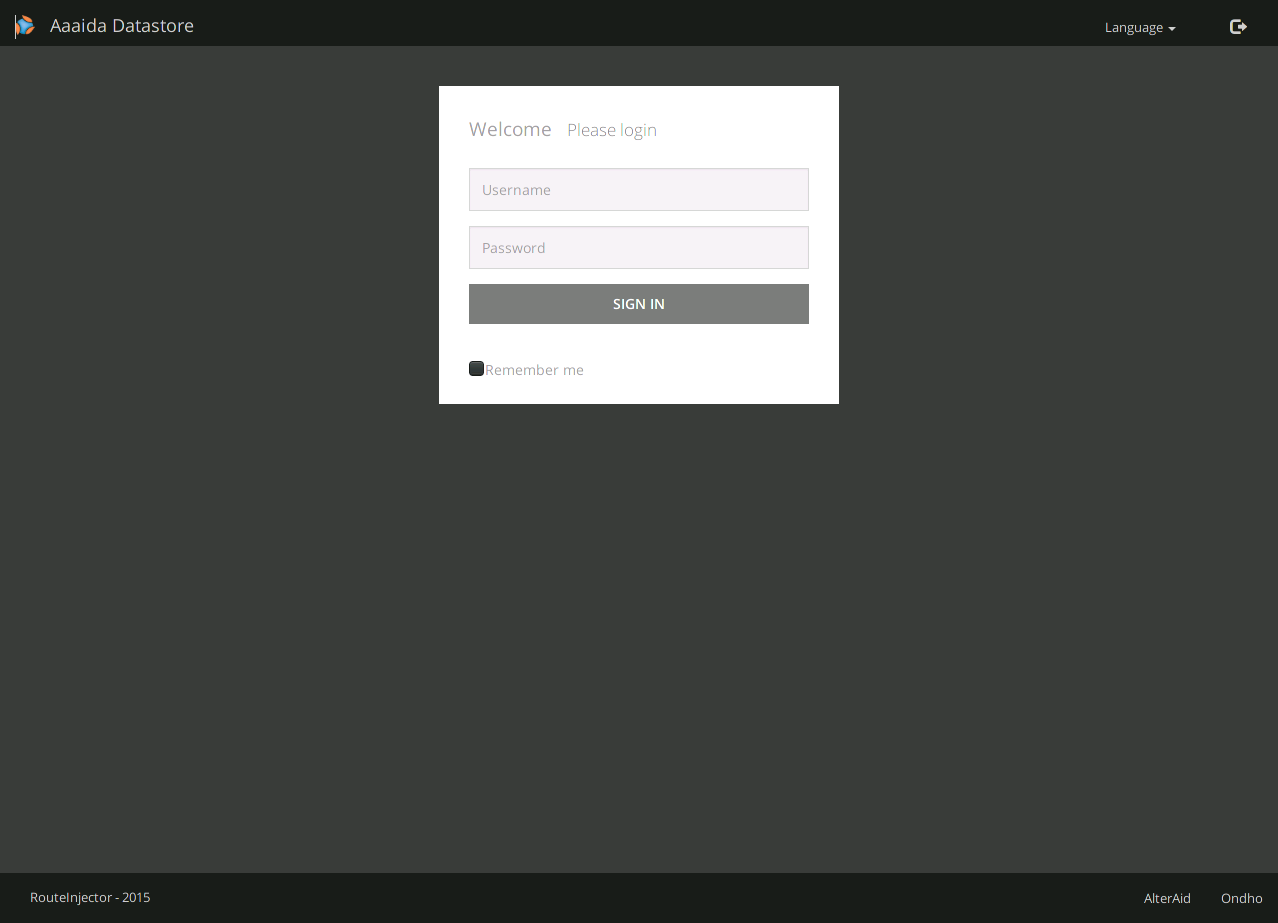
\includegraphics[width=0.95\textwidth]{./setup/AaaidaDatastore}
\caption{Acceso a Aaaida}
\label{webLog:LoggeoAaaida}
\end{center}
\end{figure} 

La base de datos está vacía. Al no tener datos no hay usuarios por lo tanto  no se podrá acceder a la plataforma de Aaaida, la solución es cargar un dump de la base de datos en el contenedor de \texttt{mongo} para que éste encuentre los datos y poder acceder a la plataforma.  Para hacer el volcado de datos es necesario saber la IP del contenedor ya que será la manera de decir donde queremos hacer el restore de la base de datos. Para poder extraer información de los contenedores se utiliza el comando \texttt{docker inspect}. En la figura siguiente se verá la ejecución del comando y de donde obtendremos la IP de nuestro contenedor de mongo.
\pagebreak

\begin{figure}[htb]
\begin{center}
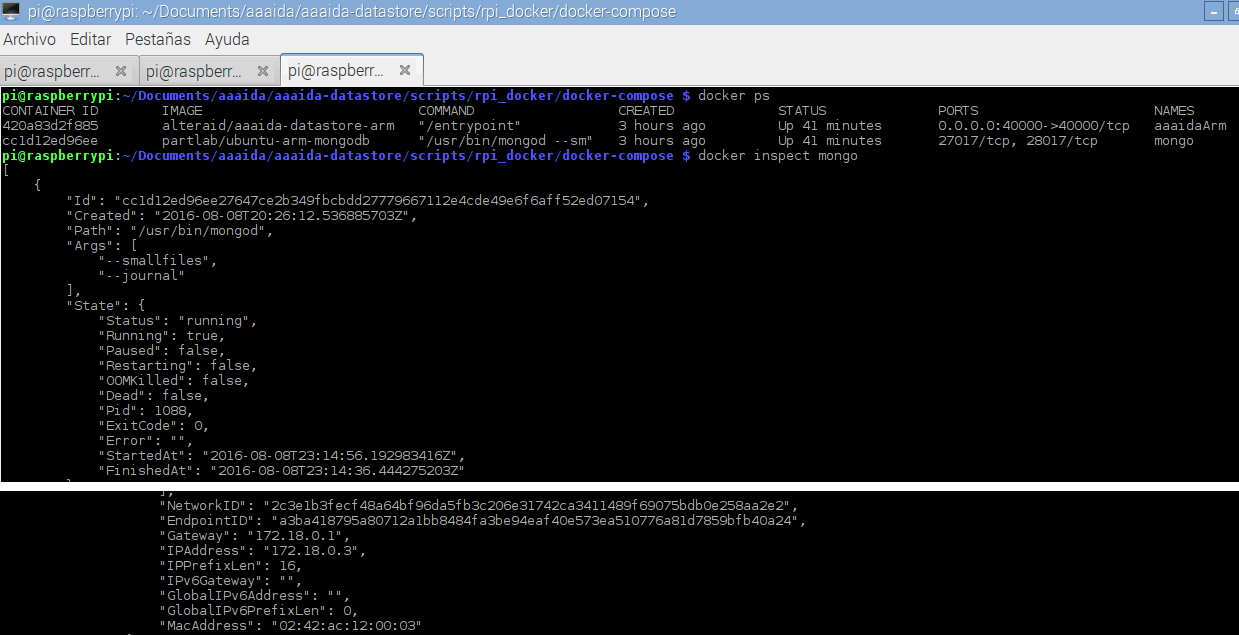
\includegraphics[width=0.95\textwidth]{./setup/dockerinspect}
\caption{Docker inspect}
\label{insp:dockerInspect}
\end{center}
\end{figure} 

Una vez se obtiene la IP del contenedor, \texttt{IPAddress: 172.18.0.3}, se ejecuta el siguiente comando para llevar a cabo el volcado de datos:

\begin{center}
\texttt{mongorestore dump/ -h 172.18.0.3}
\end{center}

Una vez disponemos de todas las piezas listas, se puede dar por concluido el proceso de despliegue de Aaaida en una Raspberry Pi utilizando Docker. 

\begin{figure}[htb]
\begin{center}
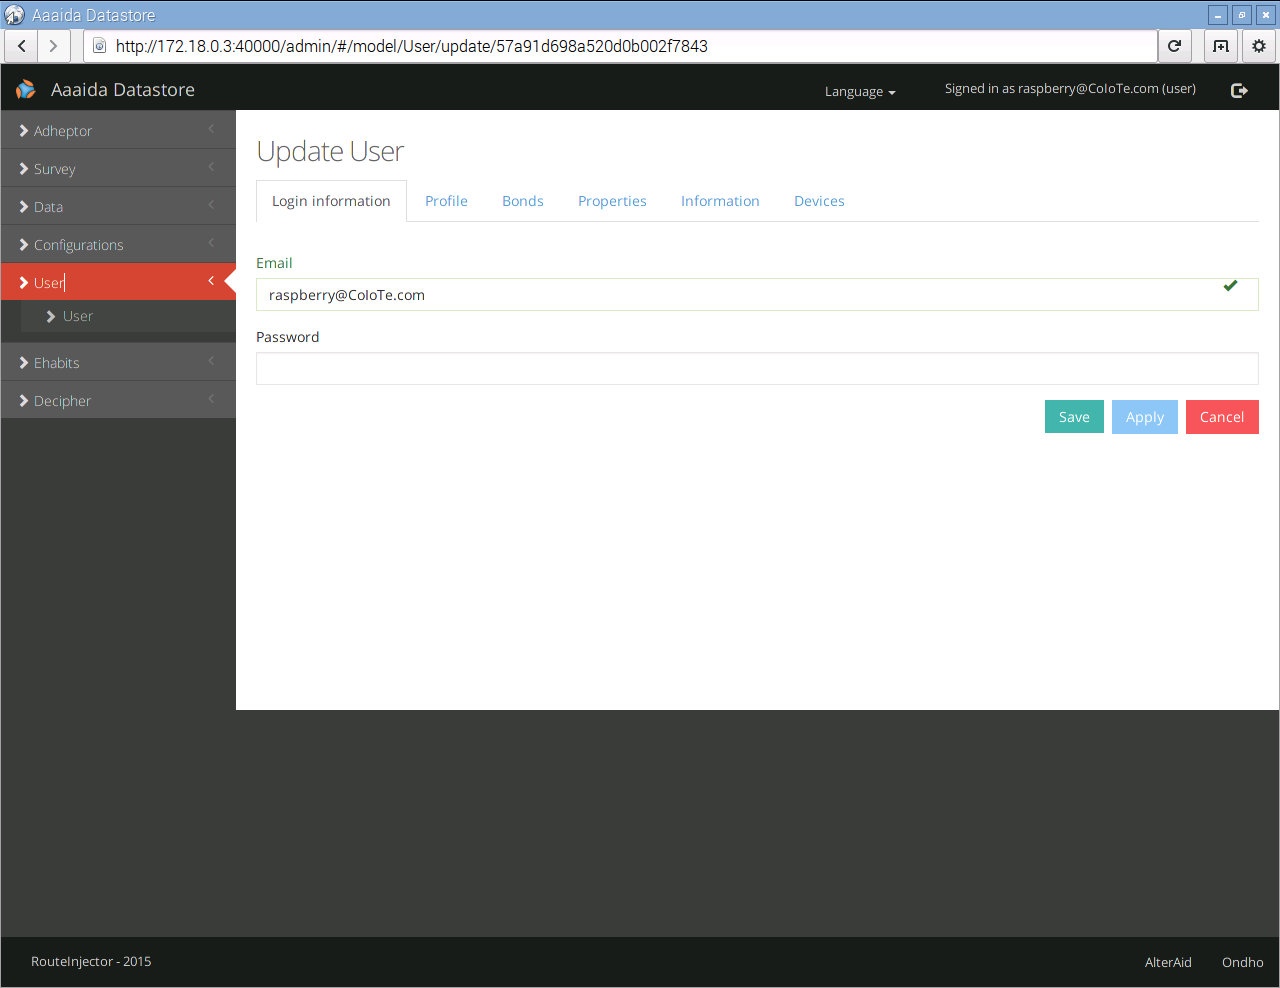
\includegraphics[width=0.70\textwidth]{./setup/aaaidaCoIoTe}
\caption{Interfaz de Aaaida}
\label{aidaCoI:aaaidaCoiote}
\end{center}
\end{figure} 
 
 \subsection{Conclusiones} 
 
En este capítulo se puede ver que la Raspberry Pi es el dispositivo para IoT más popular en el mercado, tanto por su prestaciones como por su reducido precio.
 
No es posible virtualizar la Raspberry Pi mediante Qemu y utilizar Docker ya que el kernel no es compatible. 

Y por último, aunque Docker no sea compatible para un sistema ARM gracias a unos pequeños cambios en la imagen sí puede ejecutar. Por lo tanto se pudo desplegar toda la infraestructura en la Raspberry Pi y Aaaida funciona perfectamente. 